% =============================================================
% Chapter 8: Result Analysis
% =============================================================

\newpage
\vspace*{\fill}
\begin{center}
\textbf{\Huge{Chapter 8}}\\
\vspace{5mm}
\textbf{\Huge{Result Analysis}}
\end{center}
$1
\begin{center}
\thepage
\end{center}
$2

\titleformat{\chapter}[block]{\normalfont}{}{0pt}{}
\titlespacing{\chapter}{0pt}{-2em}{0pt}
\chapter[Result Analysis]{}
\thispagestyle{fancy}
\renewcommand{\thefigure}{8.2}
\begin{figure}[!htbp]
    \centering
    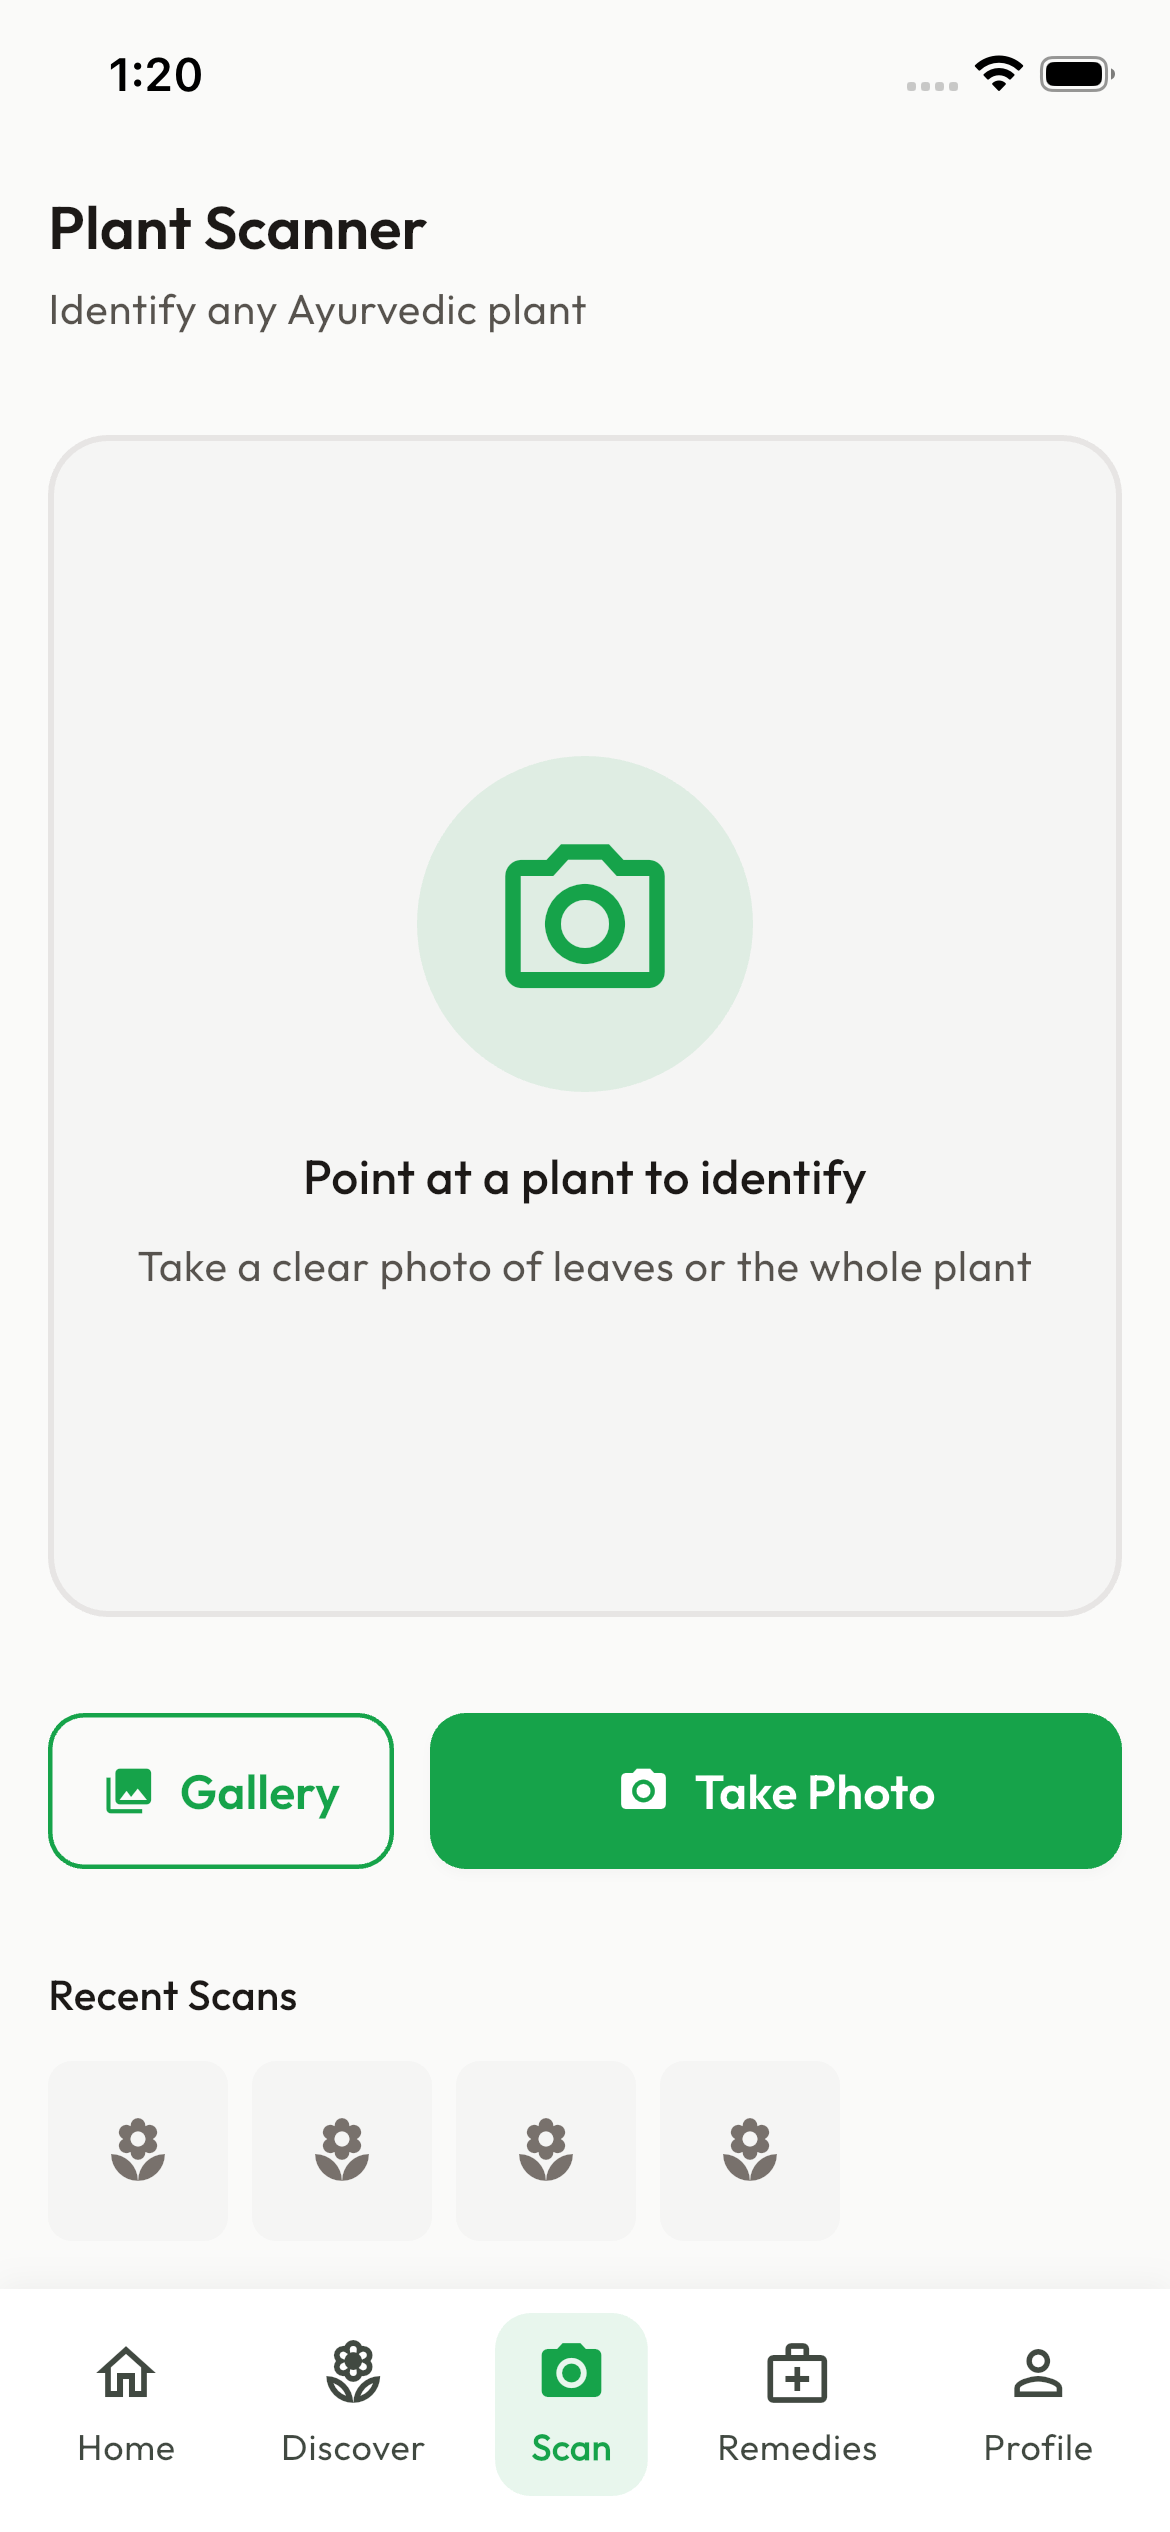
\includegraphics[width=0.3\textwidth]{screenshots/scan_plant_screen.png}
    \caption{Plant Scanning Interface}
    \label{fig:plant-scanning}

    \vspace{10pt}
    \justify
    Figure 8.2 presents the Plant Scanning Interface utilizing the device camera. The image captured here undergoes the critical pre-processing $P(I_{raw})$ downsampling before being dispatched to the Plant.id residual network over HTTP.
\end{figure}

\renewcommand{\thefigure}{8.3}
\begin{figure}[!htbp]
    \centering
    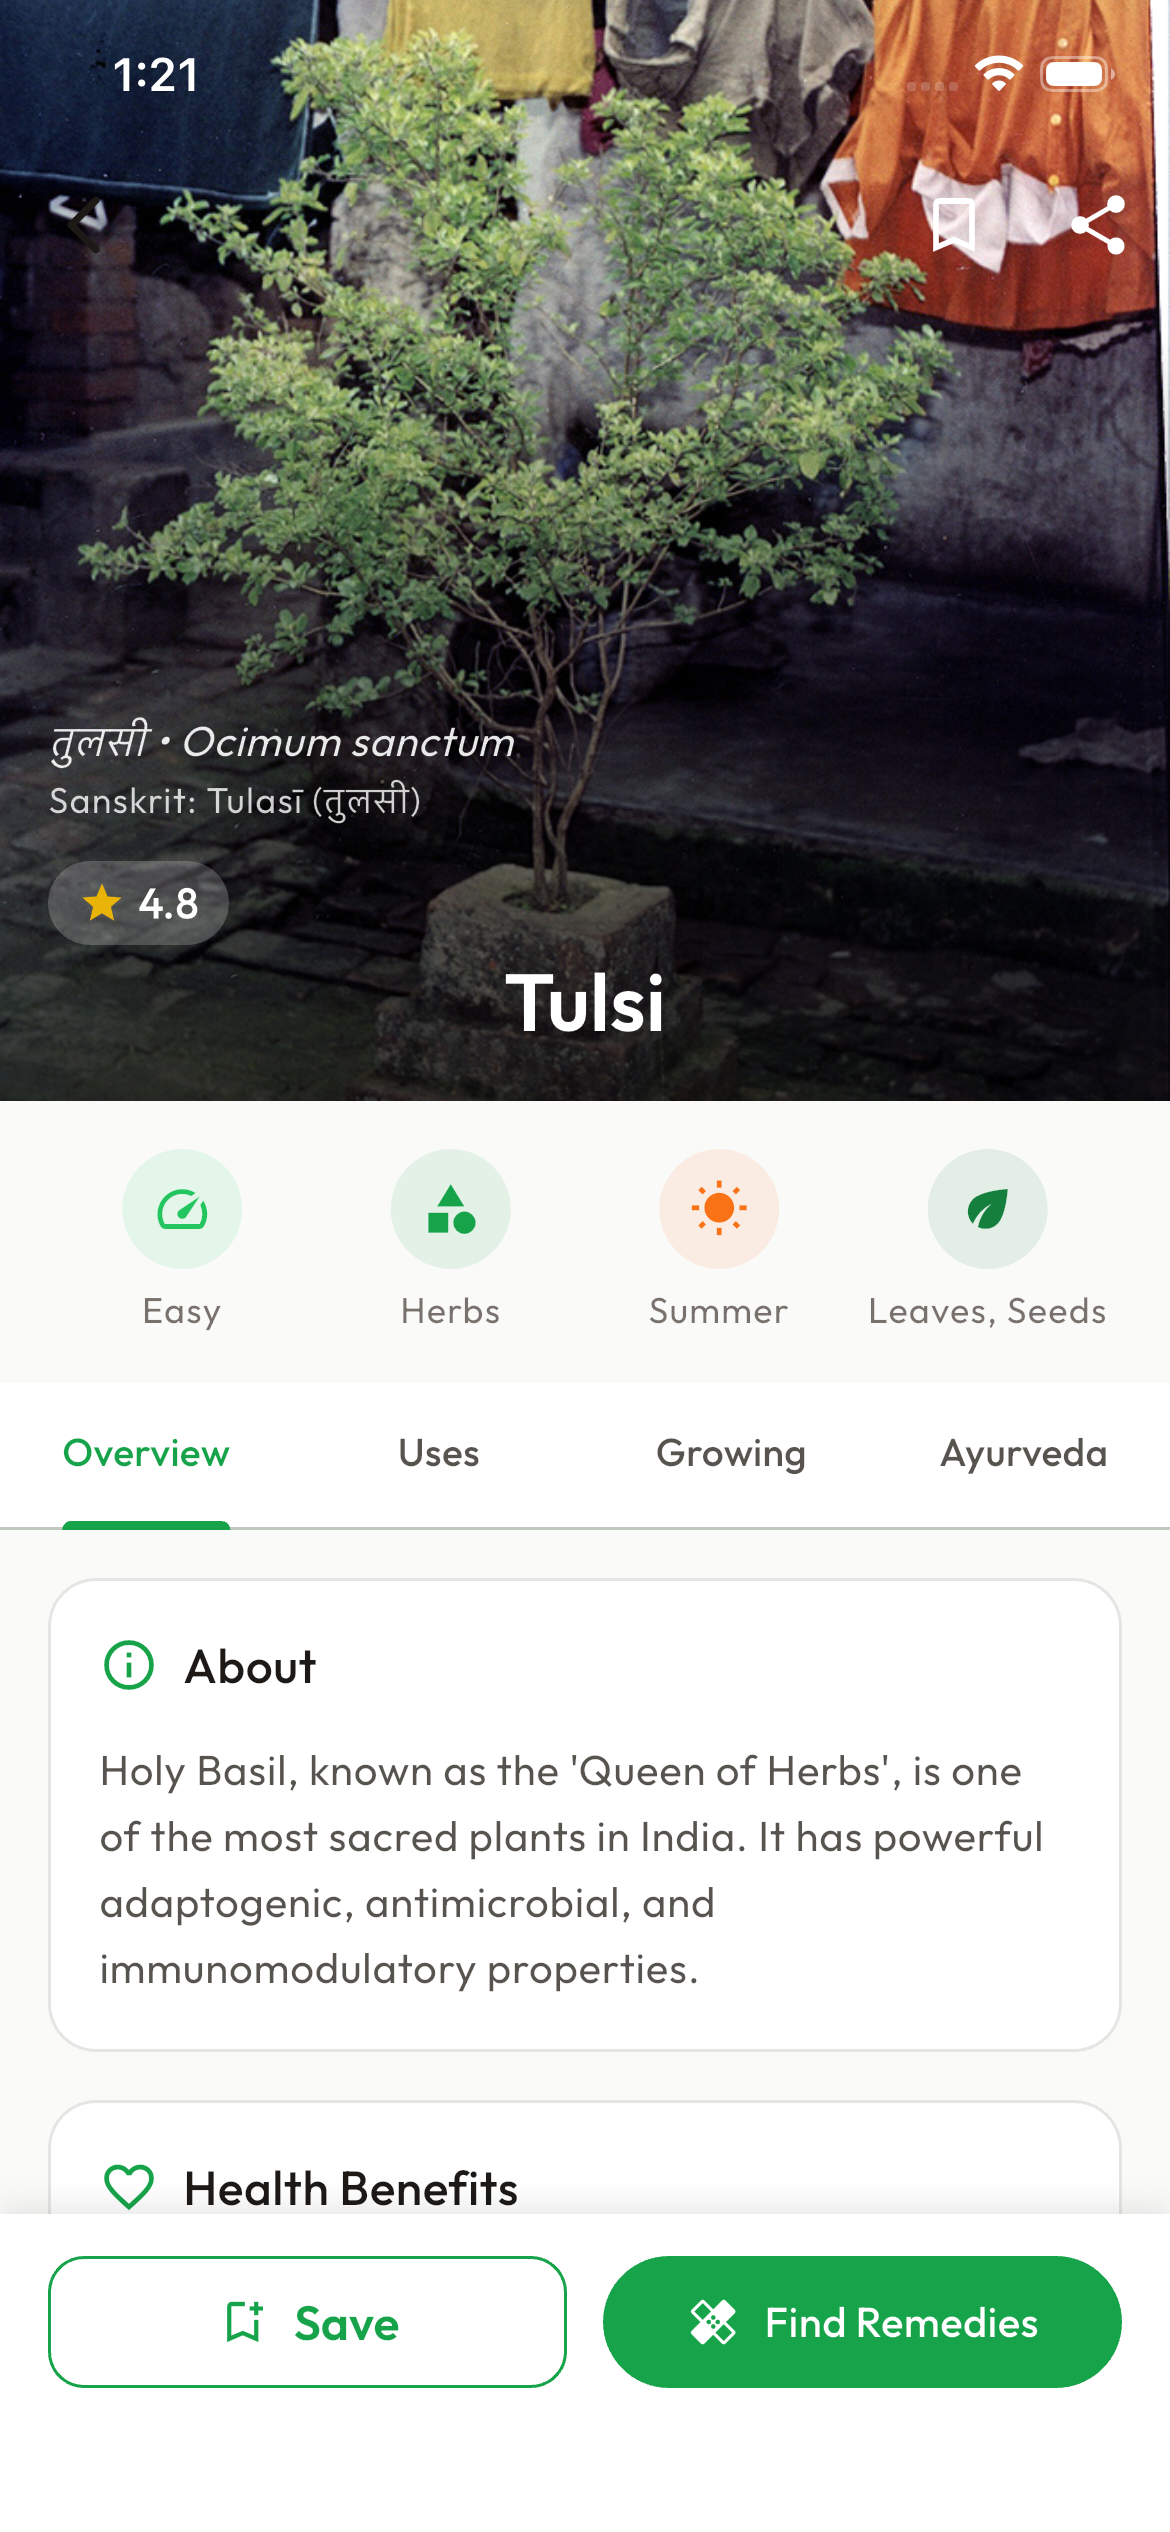
\includegraphics[width=0.3\textwidth]{screenshots/plant_detail_screen.png}
    \caption{AI Diagnostic Results and Plant Detail}
    \label{fig:plant-detail}

    \vspace{10pt}
    \justify
    Figure 8.3 showcases the comprehensive response generated after inference. It fuses the visual taxonomy from Plant.id with the \textit{Rasa, Guna, Virya}, and \textit{Vipaka} data generated contextually by the Gemini LLM.
\end{figure}

\renewcommand{\thefigure}{8.4}
\begin{figure}[!htbp]
    \centering
    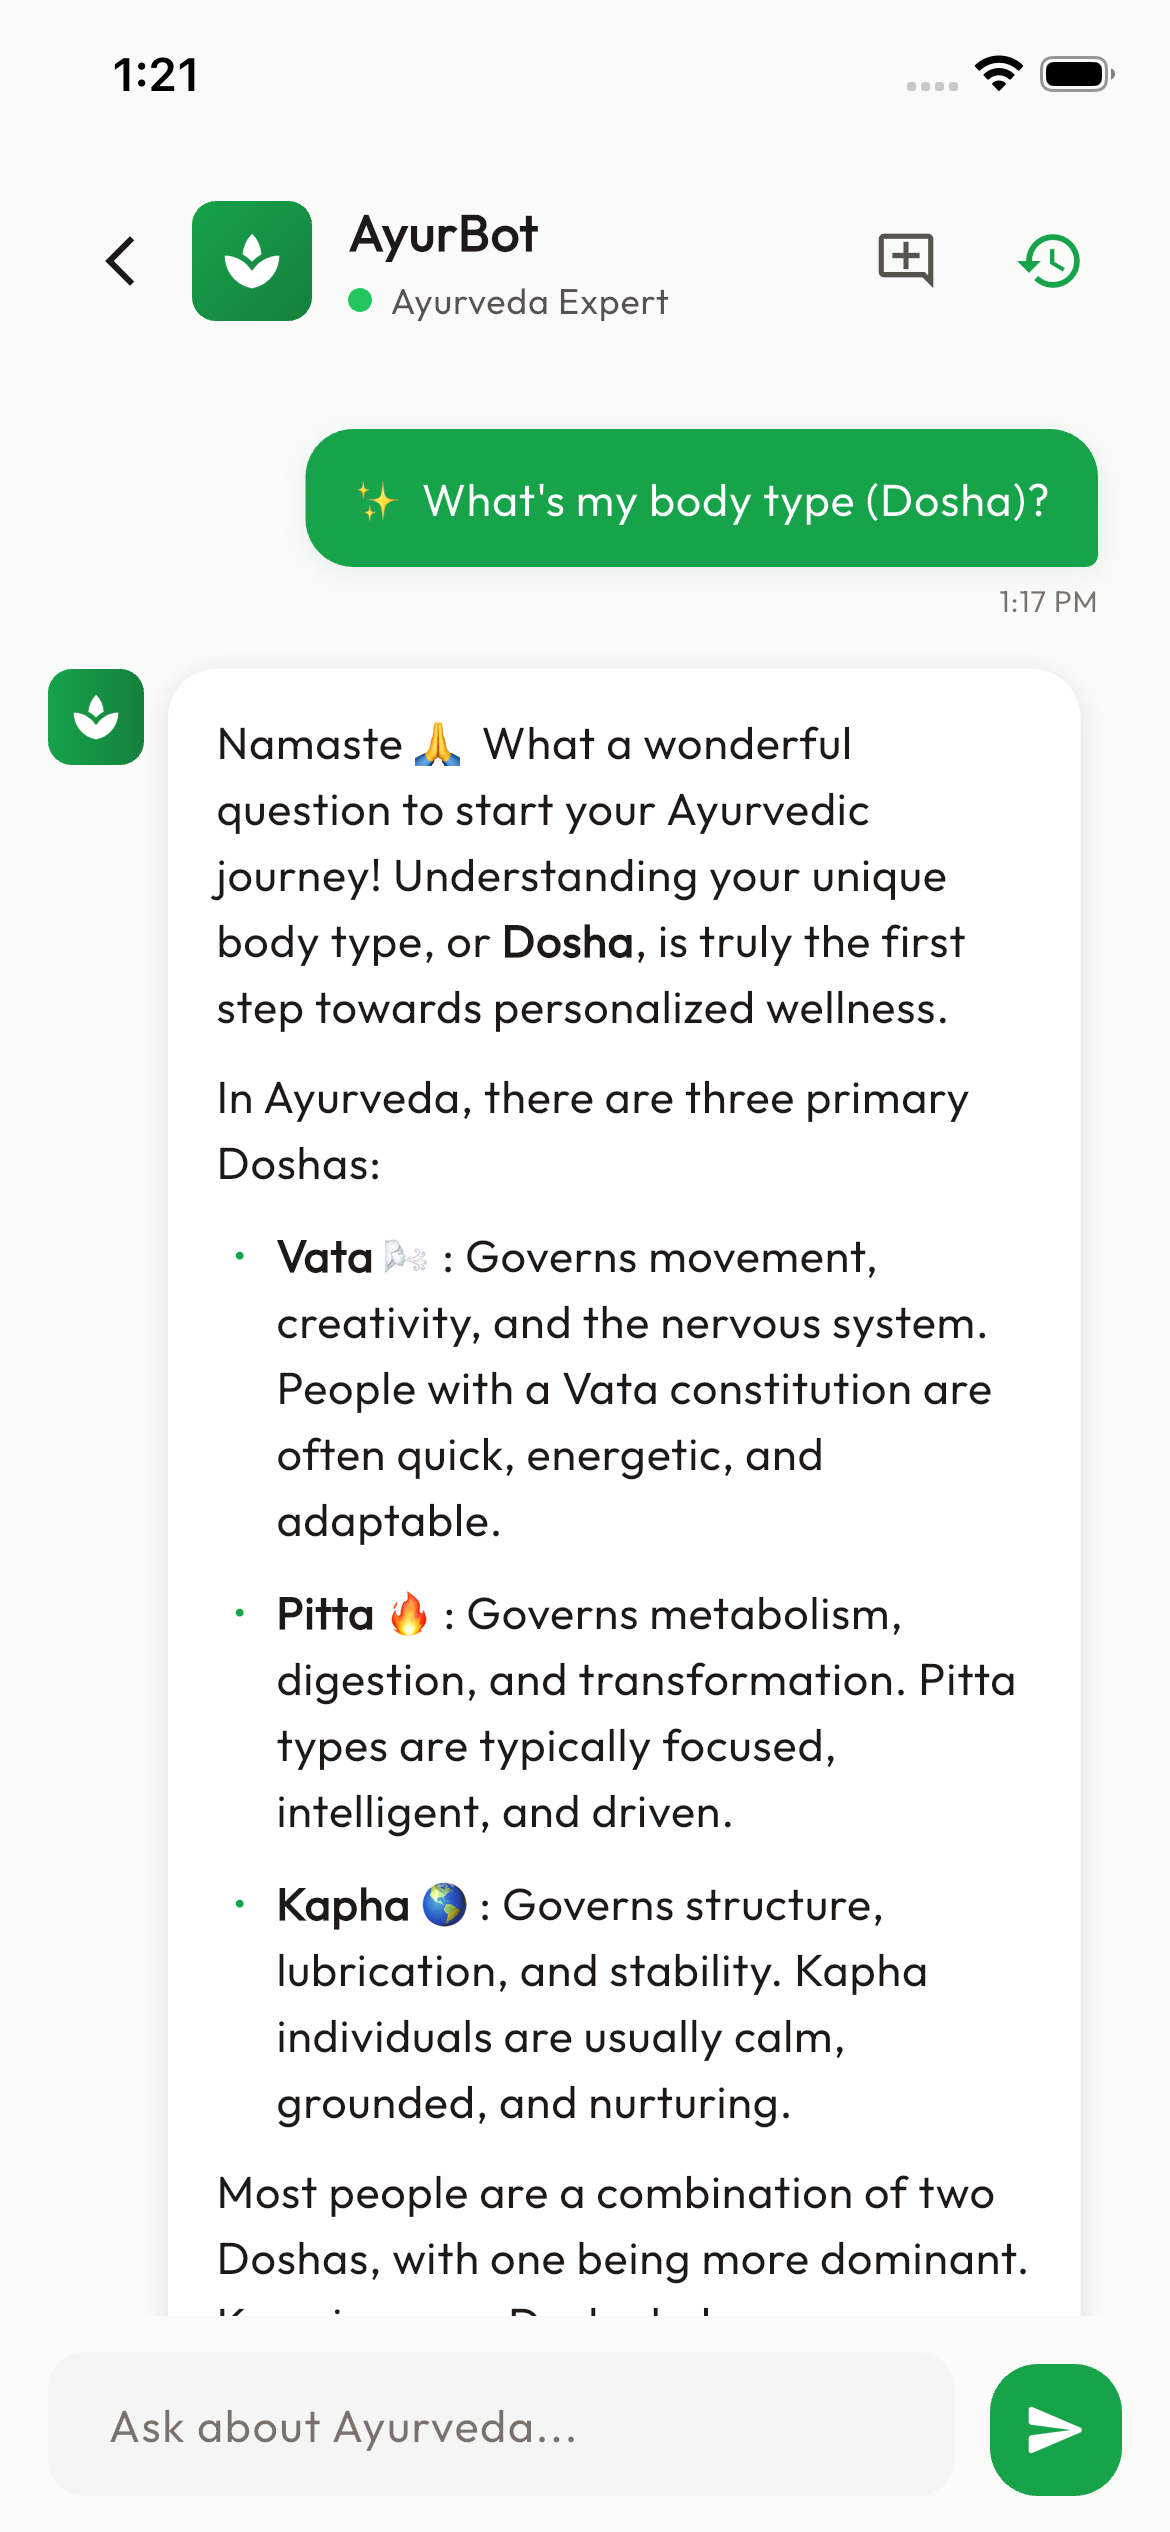
\includegraphics[width=0.3\textwidth]{screenshots/AyurBot_screen.png}
    \caption{AyurBot Chat Session}
    \label{fig:ayurbot}

    \vspace{10pt}
    \justify
    Figure 8.4 depicts a live, multi-turn chat session with AyurBot. The Riverpod \texttt{ChatNotifier} listens to the stream and renders message bubbles while safely passing the patient's dosha context silently via the System Instruction API.
\end{figure}

\renewcommand{\thefigure}{8.5}
\begin{figure}[!htbp]
    \centering
    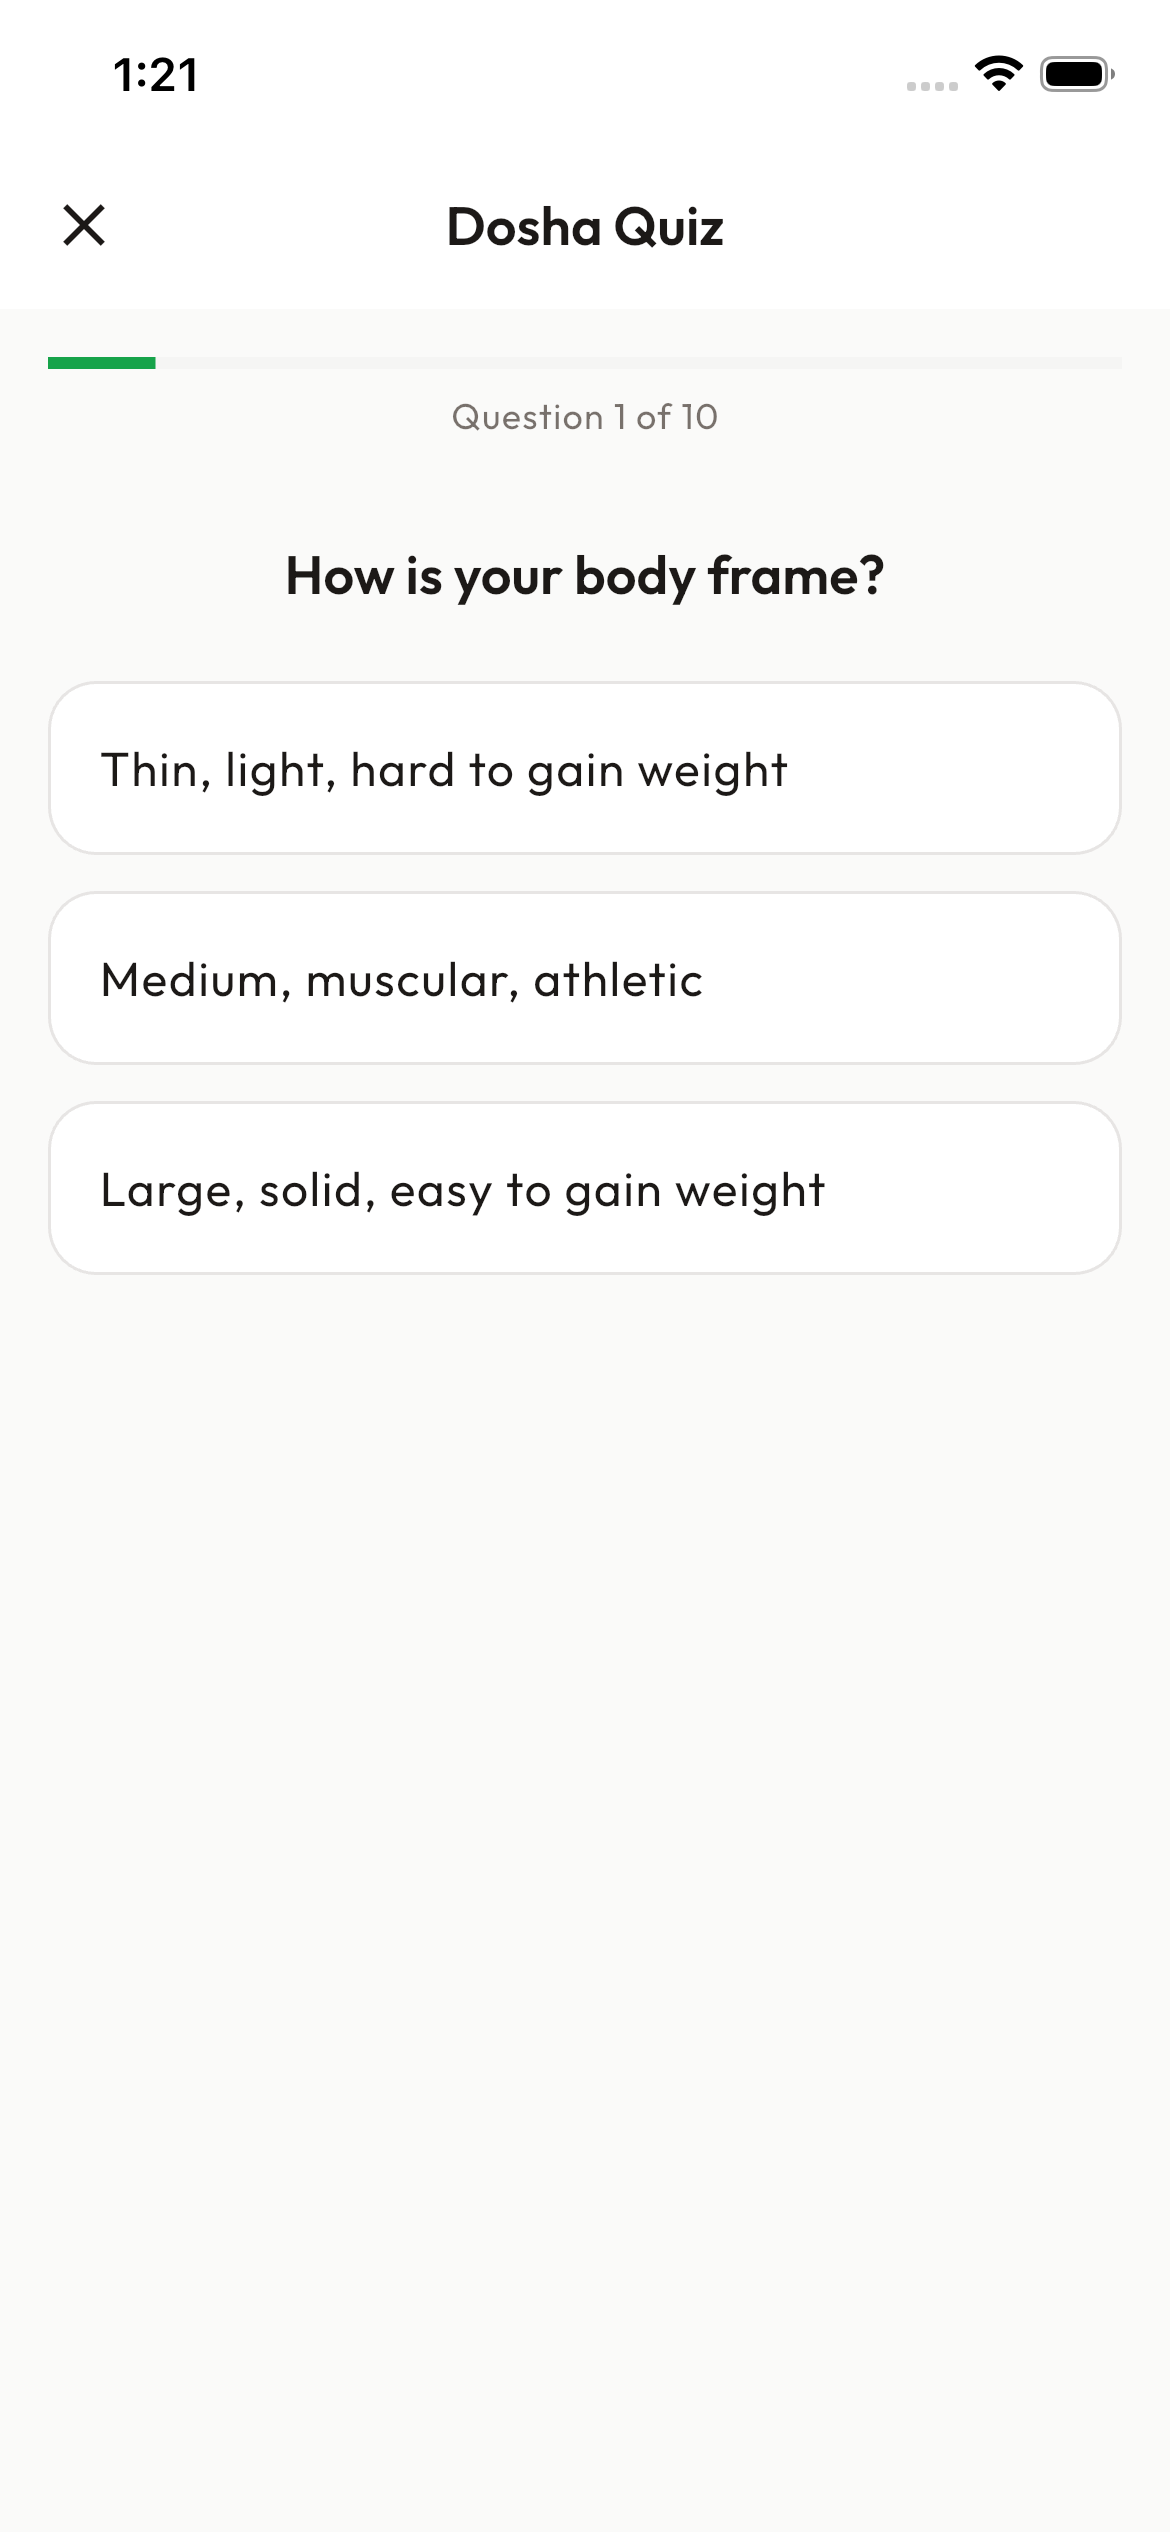
\includegraphics[width=0.3\textwidth]{screenshots/dosha_quiz_screen.png}
    \caption{Tridosha Quiz Assessment Screen}
    \label{fig:dosha-quiz}

    \vspace{10pt}
    \justify
    Figure 8.5 presents the Tridosha Quiz where the user's choices are bound to algorithmic weights, resolving into a discrete mathematical model for baseline health prediction.
\end{figure}

\newpage
\section{Experimental Setup \& Metric Definition}
To thoroughly assess the system, we set the following standards:
\begin{enumerate}
    \item \textbf{Top-1 Identification Accuracy ($Acc_1$)}: The frequency with which the ground-truth species is the first suggestion returned.
    \item \textbf{Hallucination Rate ($H_r$)}: The frequency at which the LLM generates incorrect properties for a plant that is already known.
    \item \textbf{End-to-End Latency ($L_{total}$)}: The whole time from capture to the last UI render.
\end{enumerate}

Testing was done on an Android phone (mid-range level) over a normal 4G LTE network. We tested the system with a dataset of 50 different medicinal plant species prevalent in the Indian subcontinent (e.g., \textit{Ocimum sanctum, Azadirachta indica, Tinospora cordifolia}).

\section{Performance Benchmarks}

\begin{table}[htbp]
\caption{System Performance Benchmarks}
\begin{center}
\begin{tabular}{|c|c|l|}
\hline
\textbf{Metric} & \textbf{Value} & \textbf{Notes} \\
\hline
\textbf{Plant.id Accuracy} & 96.4\% & Precision on top-1 prediction \\
\hline
\textbf{Gemini Conformance} & 99.1\% & Valid JSON schema generation \\
\hline
\textbf{Comp. Efficiency} & 85\% & Payload cut to $\approx$850KB \\
\hline
\textbf{Avg. ID Latency} & 2.1s & Plant.id API response time \\
\hline
\textbf{Avg. LLM Latency} & 1.8s & Gemini 1.5 Flash inference \\
\hline
\textbf{Total Latency} & \textbf{4.2s} & End-to-end UX threshold \\
\hline
\end{tabular}
\end{center}
\end{table}

The total system latency of 4.2s is within the range of what is acceptable for non-real-time educational apps. The image compression pipeline made a very small difference of 200ms of extra time, but saved about 1.5s in the network time it takes to send raw uploads.

\section{Ablation Study}
We compared our Neuro-Symbolic method to a pure multimodal approach from start to finish.
\begin{itemize}
    \item \textbf{Pathway A (Control)}: Send image directly to Gemini Vision Pro. Analysis: Not clear. Sometimes gets plants wrong.
    \item \textbf{Pathway B (AyurSpace Hybrid)}: Plant.id + Gemini. Analysis: Exact, medically correct, and strictly structured.
\end{itemize}
\textbf{Conclusion}: Specialized Narrow AI (Vision) combined with Generalized AI (Reasoning) significantly outperforms Generalized Multi-modal AI alone for this specific architectural area.
